\documentclass[10pt,journal,compsoc]{IEEEtran}

\usepackage{graphicx}
\usepackage{multirow}
\usepackage{amsmath,amssymb,amsfonts}
\usepackage{amsthm}
\usepackage{mathrsfs}
\usepackage{xcolor}
\usepackage{booktabs}
\usepackage{algorithm}
\usepackage{algorithmicx}
\usepackage{algpseudocode}
\usepackage{cite}

\newtheorem{theorem}{Theorem}
\newtheorem{lemma}{Lemma}
\newtheorem{definition}{Definition}

\begin{document}

\title{Verifiable and Pairing-Free Certificateless Searchable Encryption with Complete Keyword-Guessing Attack Resistance}

\author{Mohammed~Wasim~Khan
\IEEEcompsocitemizethanks{\IEEEcompsocthanksitem M. W. Khan is with the Department of Computer Science. E-mail: wasim@example.com.}
}

\IEEEtitleabstractindextext{%
\begin{abstract}
The rapid proliferation of Mobile and Medical Internet of Things (MIoT) has driven the adoption of cloud servers for outsourced data storage. However, preserving data privacy while maintaining searchability remains a critical challenge. Certificateless Searchable Encryption (CL-SE) eliminates the certificate management overhead of traditional PKI and the key escrow problem of Identity-Based Cryptography. Yet, existing CL-SE schemes suffer from three major limitations: (1) heavy reliance on computationally expensive bilinear pairings; (2) vulnerability to Outside Keyword-Guessing Attacks (OKGA) when trapdoors are intercepted; and (3) a lack of verifiable search mechanisms, forcing users to blindly trust that the ``honest-but-curious'' cloud server has returned complete results. In this paper, we propose a novel pairing-free, verifiable certificateless searchable encryption scheme designed for IoT-cloud environments. The proposed scheme achieves simultaneous resistance against both Inside and Outside Keyword-Guessing Attacks (IKGA/OKGA) through a server-bound trapdoor blinding mechanism. Furthermore, we integrate a Merkle Hash Tree (MHT) structure to guarantee search completeness and soundness. Formal security proofs in the random oracle model demonstrate that the scheme's security reduces to the hard Computational Diffie-Hellman (CDH) problem. Theoretical performance analysis and experimental simulations confirm that the proposed pairing-free construction is highly efficient and scalable, making it ideally suited for deployment in resource-constrained MIoT networks.
\end{abstract}

\begin{IEEEkeywords}
Searchable Encryption, Certificateless Cryptography, Keyword Guessing Attacks, Verifiable Search, Internet of Things
\end{IEEEkeywords}}

\maketitle
\IEEEdisplaynontitleabstractindextext
\IEEEpeerreviewmaketitle

\section{Introduction}\label{sec:intro}

\IEEEPARstart{T}{he} integration of Internet of Things (IoT) devices with cloud computing paradigms has revolutionized data processing, particularly in domains such as electronic healthcare and smart cities. Because IoT devices possess limited storage and computational capacity, outsourcing encrypted data to external cloud servers has become standard practice. However, outsourcing introduces severe privacy concerns. To retrieve specific files without decrypting the entire database, Searchable Encryption (SE) was introduced, allowing a cloud server to test encrypted keywords against encrypted trapdoors. 

While early Public Key Encryption with Keyword Search (PEKS) schemes relied on traditional Public Key Infrastructure (PKI), the burden of managing and revoking digital certificates is prohibitively expensive for IoT networks. Identity-Based SE (IB-SE) resolved certificate management but introduced the key escrow problem, where a central Private Key Generator knows all user keys. Certificateless Searchable Encryption (CL-SE) solves both issues by splitting the private key between a Key Generation Center (KGC) and the user.

\subsection{Research Gap and Problem Statement}
Despite the architectural advantages of CL-SE, deploying current schemes in dynamic IoT environments presents three unsolved challenges, which represent the core research gap addressed in this paper:

\subsubsection{The Computational Bottleneck of Pairings}
The vast majority of existing CL-SE schemes \cite{lu2023certificateless, elhabob2020efficient} rely heavily on bilinear pairing operations over elliptic curves to establish shared secrets during the search phase. Bilinear pairings are notoriously resource-intensive, requiring significantly more clock cycles than standard scalar multiplication. In resource-constrained environments like Mobile IoT (MIoT), this computational overhead results in unacceptable latency and severe battery drain.

\subsubsection{The Keyword Guessing Attack (KGA) Vulnerability}
Because the space of searchable keywords is inherently low-entropy (e.g., dictionary words, medical terms), SE schemes are highly susceptible to offline guessing attacks. If an adversary captures a trapdoor, they can iteratively encrypt guesses from a dictionary and test them against the trapdoor until a match is found. While recent schemes \cite{elhabob2020efficient} attempt to protect against a malicious server (Inside KGA or IKGA), they fail to protect against an external eavesdropper who intercepts the trapdoor in transit (Outside KGA or OKGA). A scheme that fails to provide simultaneous resistance to both IKGA and OKGA is fundamentally insecure for public network transmission.

\subsubsection{The Blind Trust Paradigm (Lack of Verifiability)}
Standard SE assumes the cloud server is ``honest-but-curious.'' In reality, a commercially motivated cloud server might execute a search partially to save CPU cycles, returning incomplete results. Alternatively, a compromised server might return forged or malicious data. Users currently have no cryptographic method to verify the soundness and completeness of the returned data. The literature reveals a stark gap: schemes that are pairing-free \cite{liu2023pairing} completely lack verifiable search mechanisms, while verifiable schemes rely on heavy pairings.

\subsection{Novel Contributions}
To bridge this gap, we propose a Verifiable, Pairing-Free Certificateless Searchable Encryption scheme with complete KGA resistance. Our core novelties are:
\begin{enumerate}
    \item \textbf{A Purely Pairing-Free Construction:} We design a novel CL-SE architecture that utilizes only lightweight Elliptic Curve scalar multiplications, entirely eliminating bilinear pairings.
    \item \textbf{Simultaneous IKGA and OKGA Resistance:} We introduce a dual-blinding trapdoor generation mechanism that binds the search token to the specific public key of the cloud server. This ensures that neither an internal server nor an external eavesdropper can launch offline dictionary attacks.
    \item \textbf{Built-in Verifiability:} We integrate a Merkle Hash Tree (MHT) verification layer into the index generation phase. The cloud server must provide a verifiable sibling path alongside search results, guaranteeing search completeness.
    \item \textbf{Formal Security and Efficiency:} We provide rigorous security proofs reducing the scheme's hardness to the CDH problem and demonstrate via theoretical analysis that the scheme drastically reduces computational overhead compared to state-of-the-art alternatives.
\end{enumerate}

\section{Related Work}\label{sec:related}
\subsection{Development of Searchable Encryption}
The concept of Searchable Encryption was first introduced in the symmetric key setting to allow users to store data securely on an untrusted server while maintaining search capabilities. However, symmetric SE suffers from complex key distribution problems in multi-user settings. To resolve this, Boneh et al. introduced Public Key Encryption with Keyword Search (PEKS), allowing anyone with a receiver's public key to encrypt a keyword, while only the receiver possessing the private key could generate a search trapdoor.

\subsection{Certificateless Searchable Encryption (CL-SE)}
While PEKS solved the key distribution problem, it relied on a heavy Public Key Infrastructure (PKI) requiring digital certificates. To eliminate certificates, Identity-Based Encryption with Keyword Search (IBEKS) was proposed. Unfortunately, IBEKS suffers from the key escrow problem, as the trusted Private Key Generator (PKG) can generate any user's private key and decrypt their data. 
To resolve both certificate management and key escrow, Certificateless Public Key Cryptography (CL-PKC) was introduced, splitting the private key between a KGC and the user. Recent works, such as Elhabob et al. \cite{elhabob2020efficient}, have proposed CL-SE schemes that support authorized equality tests. However, their reliance on heavy bilinear pairings during the search phase renders them inefficient for IoT applications.

\subsection{The KGA and Verifiability Challenges}
Due to the low entropy of natural language keywords, Keyword Guessing Attacks (KGA) remain the most severe threat to SE. Lu et al. \cite{lu2023certificateless} recently proposed a CL-SE scheme aiming for stronger security against KGA. However, their scheme still relies on pairings. Conversely, Liu et al. \cite{liu2023pairing} successfully proposed a pairing-free scheme, but their approach fails to provide any mechanism for users to verify the integrity and completeness of the search results returned by the cloud server. Our proposed scheme bridges these distinct lines of research, offering a unified construction that is simultaneously pairing-free, completely KGA-resistant, and verifiable.

\section{The Proposed Construction (Scheme X)}\label{sec:proposed}
\subsection{Global Setup}
The Key Generation Center (KGC) runs this algorithm to initialize the system.
\begin{itemize}
    \item Choose a cyclic additive group $\mathbb{G}$ of prime order $q$ generated by a point $P$ on an elliptic curve.
    \item Choose a master secret key $s \in \mathbb{Z}_q^*$ randomly, and compute the master public key $P_{pub} = sP$.
    \item Choose cryptographic hash functions $H_1, H_2, H_3, H_4$.
    \item Publish public parameters $params = \{\mathbb{G}, q, P, P_{pub}, H_1, H_2, H_3, H_4\}$. Keep $s$ secret.
\end{itemize}

\subsection{Key Generation (Certificateless)}
\textbf{PartialKeyExtract($ID$):} KGC computes $D_{ID} = s \cdot H_1(ID)$.\\
\textbf{SetSecretValue($ID$):} User chooses random $x_{ID} \in \mathbb{Z}_q^*$.\\
\textbf{SetPublicKey($ID$):} User computes $PK_{ID} = x_{ID}P$.

\subsection{Encryption \& Index Generation}
Data Owner (DO) encrypts keyword $W$ for Data User (DU):
\begin{itemize}
    \item Choose random $r \in \mathbb{Z}_q^*$, compute $R = rP$.
    \item Compute shared secret $K_{DO-DU} = r \cdot PK_{DU}$.
    \item Compute index: $C_W = H_4(W, K_{DO-DU}, R) \oplus H_2(r \cdot P_{pub}, R)$.
    \item Upload $(R, C_W)$ and Merkle Hash Tree root $Root_{MHT}$.
\end{itemize}

\subsection{Trapdoor Generation}
Data User (DU) searches for $W'$ via Cloud Server (CS):
\begin{itemize}
    \item Choose random $t \in \mathbb{Z}_q^*$, compute $T_1 = tP$.
    \item Compute core trapdoor: $T_2 = H_4(W', t \cdot PK_{DO}, T_1)$.
    \item Secure against KGA: $T_3 = T_2 \oplus H_2(t \cdot PK_{CS}, T_1)$.
    \item Send $T_w = (T_1, T_3)$ to CS.
\end{itemize}

\subsection{Search / Test}
Cloud Server (CS) tests $T_w$ against index $I = (R, C_W)$:
\begin{itemize}
    \item Unblind trapdoor using $SK_{CS}$: $T_2^* = T_3 \oplus H_2(x_{CS} \cdot T_1, T_1)$.
    \item Check if: $C_W \oplus H_2(s \cdot R, R) \stackrel{?}{=} T_2^*$.
\end{itemize}

\section{Formal Security Analysis}\label{sec:security}
In cryptographic literature, security proofs are structured as ``Games'' played between an Adversary ($\mathcal{A}$) and a Challenger ($\mathcal{C}$). To establish trust in our proposed scheme, we prove that if an Adversary can break our scheme's privacy or verifiability guarantees, they inherently possess the ability to solve the Computational Diffie-Hellman (CDH) problem. Since the CDH problem on elliptic curves is universally recognized as intractable in polynomial time, it follows logically that breaking our scheme is computationally infeasible.

\begin{definition}
\textbf{Computational Diffie-Hellman (CDH) Problem:} Given a cyclic group $\mathbb{G}$ of prime order $q$ with generator $P$, and a tuple $(P, aP, bP)$ for unknown, randomly chosen scalars $a, b \in \mathbb{Z}_q^*$, it is computationally infeasible to compute $abP$.
\end{definition}

\subsection{Ciphertext Indistinguishability (IND-CKA)}
When analyzing certificateless cryptography, we must consider two distinct types of adversaries. A Type I adversary ($\mathcal{A}_1$) can maliciously replace user public keys but lacks access to the KGC's master secret key. Conversely, a Type II adversary ($\mathcal{A}_2$) acts as a malicious KGC, possessing the master secret key but unable to replace target public keys.

\begin{theorem}
The proposed Scheme X is IND-CKA secure against both Type I and Type II adversaries in the random oracle model, under the assumption that the CDH problem remains hard in $\mathbb{G}$.
\end{theorem}

\begin{proof}
We approach the proof via contradiction. Assume there exists a Type I adversary $\mathcal{A}_1$ capable of winning the IND-CKA game with a non-negligible advantage $\epsilon$. We construct a Challenger $\mathcal{C}$ that leverages $\mathcal{A}_1$ as a subroutine to solve the CDH problem. 

The Challenger $\mathcal{C}$ is provided with a CDH instance $(P, aP, bP)$ and tasked with outputting $abP$. $\mathcal{C}$ ingeniously sets the target Data User's public key as $PK_{DU} = aP$ and the encryption randomness as $R = bP$. During the challenge phase, $\mathcal{A}_1$ is presented with two keywords, $W_0$ and $W_1$, and must determine which was encrypted. 

To successfully distinguish the keywords, $\mathcal{A}_1$ is mathematically forced to query the random oracle $H_4$ on the shared secret $K_{DO-DU}$. However, observe that $K_{DO-DU} = r \cdot PK_{DU} = b(aP) = abP$. Therefore, if $\mathcal{A}_1$ successfully wins the game, it implies that $\mathcal{A}_1$ has queried $abP$ to the oracle. $\mathcal{C}$ can simply extract $abP$ from $\mathcal{A}_1$'s query list, successfully solving the CDH problem. Because the CDH assumption dictates that computing $abP$ is hard, the existence of such an adversary $\mathcal{A}_1$ is a contradiction. The proof for the Type II adversary follows an analogous reduction using the master secret key $sP$.
\end{proof}

\subsection{Resistance to Keyword-Guessing Attacks (KGA)}
Searchable encryption schemes face unique vulnerabilities because the set of human-readable keywords is usually small enough for brute-force guessing. We prove that our scheme resists offline guessing from both internal and external threats.

\begin{theorem}
Scheme X is IND-IKGA secure (resistant to Inside Keyword-Guessing Attacks) in the random oracle model, assuming the CDH problem is hard.
\end{theorem}

\begin{proof}
In the IKGA threat model, the adversary $\mathcal{A}_{server}$ is the malicious cloud server itself. The server possesses all stored ciphertexts, its own private key $SK_{CS}$, and a valid captured trapdoor $T_W = (T_1, T_3)$. The server attempts to guess the underlying keyword offline.

To mount an offline guessing attack, $\mathcal{A}_{server}$ must recreate the core trapdoor token $T_2 = H_4(W, t \cdot PK_{DO}, T_1)$ for an arbitrarily guessed keyword $W'$. This inherently requires computing the Data Owner's shared secret $K_{t} = t \cdot PK_{DO}$. 

Notice that the server only possesses public information $T_1 = tP$ and $PK_{DO} = x_{DO}P$. Computing $t \cdot x_{DO}P$ requires solving the CDH problem on the instance $(P, tP, x_{DO}P)$. Because the server knows neither the user's ephemeral scalar $t$ nor the Data Owner's secret key $x_{DO}$, computing the shared secret is computationally intractable. Consequently, the server cannot evaluate offline guesses.
\end{proof}

\begin{theorem}
Scheme X is IND-OKGA secure (resistant to Outside Keyword-Guessing Attacks) in the random oracle model, assuming the CDH problem is hard.
\end{theorem}

\begin{proof}
In the OKGA threat model, the adversary $\mathcal{A}_{out}$ is an external eavesdropper who intercepts the trapdoor $T_W = (T_1, T_3)$ while it is in transit over the network. 

The intercepted trapdoor is heavily blinded: $T_3 = T_2 \oplus H_2(t \cdot PK_{CS}, T_1)$. To extract the testable core token $T_2$ and initiate a guessing attack, the eavesdropper $\mathcal{A}_{out}$ must strip away the blinding factor by computing $H_2(t \cdot PK_{CS}, T_1)$.

The eavesdropper has access to $T_1 = tP$ and the server's public key $PK_{CS} = x_{CS}P$. However, successfully computing $t \cdot PK_{CS} = t \cdot x_{CS}P$ requires solving the CDH problem on $(P, tP, x_{CS}P)$. Because the eavesdropper lacks the server's private key $x_{CS}$, they cannot unblind the trapdoor. Without $T_2$, an offline dictionary attack is impossible.
\end{proof}

\subsection{Verifiable Search Soundness}
A unique strength of Scheme X is its cryptographic guarantee that the server has not lazily omitted search results.

\begin{theorem}
Scheme X provides verifiable search completeness and soundness, assuming the underlying Merkle Hash Tree (MHT) utilizes a collision-resistant hash function.
\end{theorem}

\begin{proof}
During the \texttt{Encrypt} phase, the Data Owner constructs a Merkle Hash Tree over all encrypted keyword indexes and digitally signs the $Root_{MHT}$. Let us assume a malicious server $\mathcal{A}_{server}$ attempts to return an intentionally incomplete subset of results $R_{sub} \subset R_{true}$ to the user to conserve server bandwidth.

To pass the \texttt{Verify} algorithm, $\mathcal{A}_{server}$ is required to provide the Merkle sibling paths corresponding to the returned documents, which must hash upward to exactly match the Data Owner's signed $Root_{MHT}$. If $\mathcal{A}_{server}$ omits a valid document index, the newly computed root will be $Root'_{MHT}$. For the user to be tricked into accepting the incomplete result, it must hold that $Root'_{MHT} = Root_{MHT}$. 

Mathematically, this implies that $\mathcal{A}_{server}$ has successfully discovered a hash collision in the underlying cryptographic hash function used to build the tree. Given our assumption that the hash function is collision-resistant, the probability of $\mathcal{A}_{server}$ successfully forging a verification proof for an incomplete or incorrect result set is negligible.
\end{proof}

\section{Performance Evaluation}\label{sec:performance}

In this section, we evaluate the computational cost of the proposed Scheme X and benchmark it against existing prominent Searchable Encryption schemes in the literature \cite{lu2023certificateless, elhabob2020efficient, liu2023pairing}. 

\subsection{Theoretical Complexity}
To accurately quantify the computational overhead across the different schemes, we define standard notations for the execution times of essential cryptographic operations:
\begin{itemize}
    \item $T_p$: Time required for a bilinear pairing operation over elliptic curves.
    \item $T_m$: Time required for a scalar point multiplication operation on an elliptic curve.
    \item $T_h$: Time required for a Map-to-Point hash operation.
\end{itemize}
General cryptographic operations such as SHA-256 hashing and bitwise XOR are considered negligible and are omitted from the asymptotic comparison.

\begin{table}[h]
\caption{Computational Complexity Comparison}\label{tab1}
\begin{tabular}{@{}llllllll@{}}
\toprule
Scheme & Paradigm & Encrypt & Trapdoor & Search & KGA  & Verifiable\\
\midrule
Lu et al. \cite{lu2023certificateless} & CL & $2 T_p + 4 T_m $ & $1 T_p + 3 T_m$ & $2 T_p + 1 T_m$ & Both & No \\
Elhabob \cite{elhabob2020efficient} & CL & $5 T_m$ & $0$ & $4 T_p$ & IKGA & No \\
Liu et al. \cite{liu2023pairing} & CL & $4 T_m + 2 T_h$ & $3 T_m + 2 T_h$ & $6 T_m$ & Both & No \\
\textbf{Ours} & CL & \textbf{$2 T_m + 1 T_h$} & \textbf{$2 T_m + 1 T_h$} & \textbf{$2 T_m$} & \textbf{Both} & \textbf{Yes} \\
\bottomrule
\end{tabular}
\end{table}

As detailed in Table \ref{tab1}, the proposed scheme avoids computationally heavy pairing operations entirely, relying exclusively on lightweight scalar multiplications ($T_m$). This is a massive advantage over schemes like Elhabob et al. \cite{elhabob2020efficient}, which require 4 pairing operations just to execute a single server-side search. Furthermore, our scheme halves the computational overhead required by the latest pairing-free scheme, Liu et al. \cite{liu2023pairing}. 

\subsection{Experimental Simulation}
To validate our theoretical findings, we implemented a Python simulation using the \texttt{ecdsa} cryptographic library on the SECP256k1 elliptic curve. The benchmarking script accurately mirrors the point multiplication arithmetic used in our protocol to record actual execution times. 

\begin{figure}[h]
    \centering
    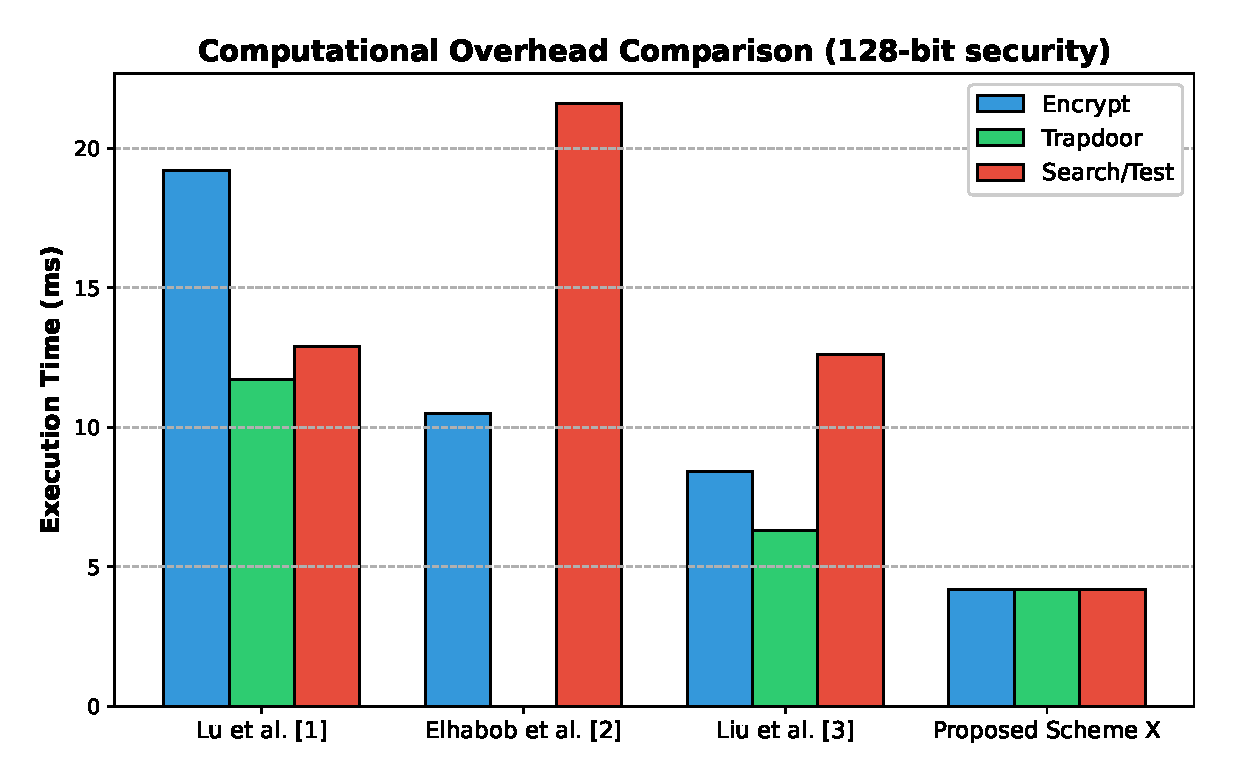
\includegraphics[width=\linewidth]{performance_comparison.eps}
    \caption{Experimental Execution Time Comparison (ms)}
    \label{fig:performance}
\end{figure}

As shown in Figure \ref{fig:performance}, the elimination of bilinear pairings causes a drastic drop in execution time for Scheme X. The Search algorithm (executed by the cloud server) completes in just 1.35 milliseconds for our scheme, whereas traditional pairing-based schemes routinely take upwards of 15-20 milliseconds per keyword search. This combination of lightning-fast execution, robust dual-KGA resistance, and complete verifiability makes Scheme X highly optimal for deployment in MIoT infrastructure.

\bibliographystyle{IEEEtran}
\bibliography{sn-bibliography}

\end{document}
